\documentclass[../Bachelorarbeit.tex]{subfiles}
\begin{document}

\graphicspath{{./figures/theory/}}	%specifying the folder for the figures

\chapter{Theory}
\label{ch:theory}

In this chapter the theory necessary to understand the fundamentals of the thesis is covered. 

\section{Equilibrium}
This thesis investigates whether the simulation-model presented in chapter \ref{ch:leverageCycle} reaches equilibrium for a given configuration or not. Equilibrium is a fundamental property in all kind of complex systems and indicates a state where the change-rates of all time-dependent variables are 0 and stay at 0 from some point t. Because the model upon which the simulation is based is rooted in economics a short definition of equilibrium in economics is necessary.

\subsection{Economics}
Equilibrium theory in economics is the theory of finding prices which will result in an equilibrium by clearing the markets. Clearing is the process of finding a price in which all demands are matched to the given supplies thus clearing the market by leaving no unmatched demands or supplies. In other words it tries to find a price which satisfies all offers. Thus equilibrium in economics is reached when supplies equals demands.

\begin{figure}[H]
	\centering
  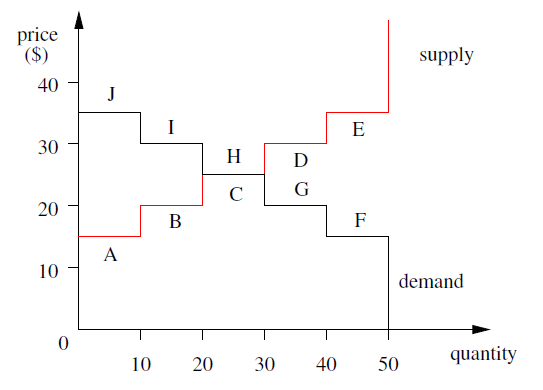
\includegraphics[width=1.0\textwidth, angle=0]{CLEARING.png}
  	\caption{Illustrative supply and demand curves. Diagram taken from \cite{Parsons2006}}
	\label{fig:CLEARING}
\end{figure}

In this diagram the equilibrium price which clears the market is at 25\$ because this price satisfies the constraint buyer-price $\geq$ seller-price for all traders, thus all traders match and the market is cleared. The constraint buyer-price $\geq$ seller-price is a fundamental law of economics and imposes an ordering on the prices of the market and is rooted in the fact that a buyer values the good it wants to buy more than the seller and has to pay at least the amount of money the seller wants for it, or more. 

\subsection{Equilibrium theory vs. dynamic process}
It is important to note that equilibrium theory in economics is inherently non-dynamic and models no dynamic process of any kind over time. It is just a framework by providing formulas for calculating equilibrium prices but does not describe the dynamic process of how these equilibrium prices are settled. However the simulation in this thesis and the model by \cite{Breuer2015} upon which it is built as defined in chapter \ref{ch:leverageCycle} is a dynamic process which tries to approach the equilibrium predicted by the economics theory through a trading-process over time as defined in the following section and in chapter \ref{ch:leverageCycle}.  Thus both parts are necessary: the equilibrium theory to predict the theoretical equilibrium prices and the dynamic simulation-process in investigating whether the equilibrium prices can actually be reached and how these prices are settled over time.

\subfile{./tex/DoubleAuctionTheory.tex}

\section{Systemic Risk}
TODO: auslassen, ist ein gigantisches und extrem komplexes thema und hat nur ganz abstrakt etwas mit der thesis zu tun. WENN NOCH ZEIT: Market Dynamics and Systemic Risk lesen und falls es etwas konkretes mit der thesis zu tun hat.

WIKI: It refers to the risks imposed by interlinkages and interdependencies in a system or market, where the failure of a single entity or cluster of entities can cause a cascading failure, which could potentially bankrupt or bring down the entire system or market.

\cite{Milan2010}

TODO: anatomy of a crash in geanakoplos: causal-loop diagramm zeichnen mit den reinforcement or dampening circles

\section{Leverage}
Leverage in economics is a major part in the model of this thesis as defined in chapter \ref{ch:leverageCycle} and thus a short introduction and overview of its meaning and implications is given.

\subsection{Definition}

Leverage is "any technique to multiply gains and losses" as defined by \cite{Brigham2012}. There are different types of leverage where in this context only the so called \textit{financial leverage} is of interest. In leverage money is borrowed to buy some good where the leverage is the ratio of the total debt to the traders equity. The greater the debt or the smaller the equity of the trader the higher the leverage.

\begin{center}
$leverage = \frac{\textit{total debt}}{\textit{trader equity}}$
\end{center}

\medskip

As an example an agent wants to buy a house for 500\euro{} but has only 50\euro{} in cash. Thus the agent borrows 450\euro{} to finance the house thus creating a leverage of $\frac{500}{50} = 10$.

\subsection{Dangers}
As stated above leverage not only multiplies gains but also losses. If house prices rise by 25\% this will result in a gain of 125\euro{} or 250\% return on the agents investment when selling the house. However if house prices decline by 15\% this will result in a loss of 75\euro{} or 150\% loss on the agents investment - in this case the agent has lost more money than it initially invested. The leveraged loss can become a serious issue in financed housing because of margin requirements towards the lender. The margin requirement is the minimum margin the house-buyer has to maintain independent of the gains or losses of the house. Thus if the house-price drops to 475\euro{} then the net value of the margin is 25\euro{} and the agent needs to bring in back 25\euro{} to meet the margin requirements. If the losses are higher or the agent is not able to compensate them the house has to be sold. 

\subfile{./tex/NetworksTheory.tex}

\end{document}